\section{Hierarchical Multi-Target Regression (HMTR)}


\begin{figure}[tb]
\hrule\vspace{1em}
\begin{verbatim}
[HMTR]
Type = Tree                        % Tree or DAG hierarchy?
Distance = WeightedEuclidean       % The distance function
Aggregation = SUM                  % The aggregation function
Weight = 0.75                      % The weight parameter w_0
Hierarchy = ALL-ECOG,ALL-ADAS13... % The HMTR hierarchy (see examples)
\end{verbatim}
\hrule
\caption{Settings specific for Hierarchical Multi-Target Regression (HMTR)}
\label{settings-hmtr:fig}
\end{figure}

\begin{figure}[tb]
\centering
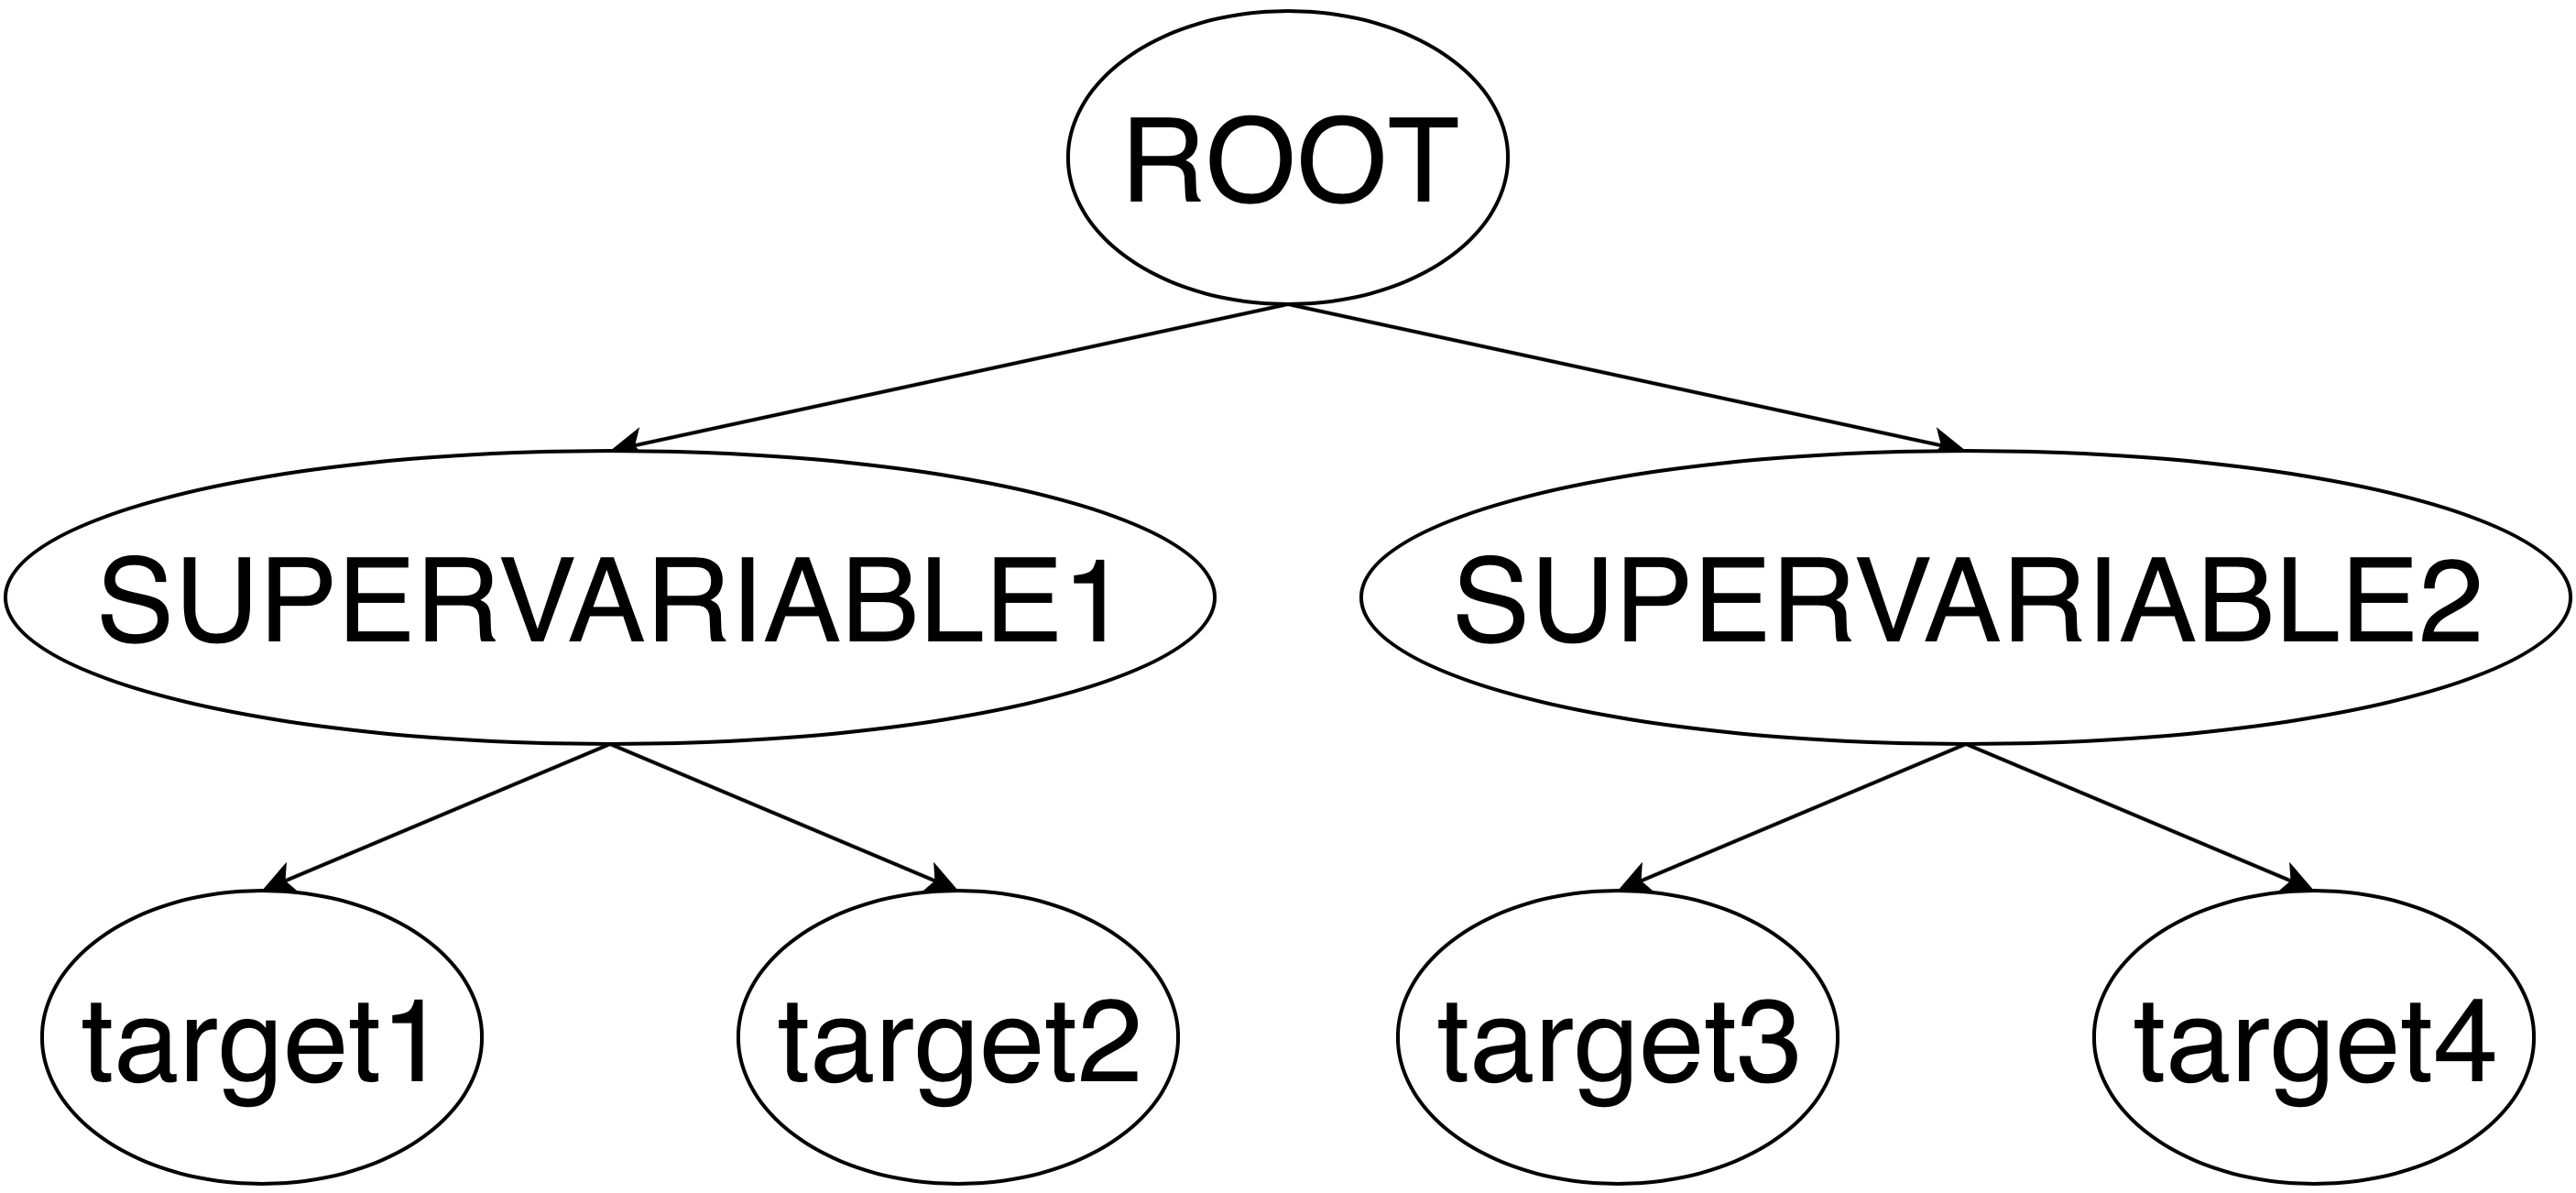
\includegraphics[width=0.5\textwidth]{fig/hmtr}
\caption{An example of a HMTR tree hierarchy.}
\label{settings-hmtrex:fig}
\end{figure}

These settings are relevant when using \clus{} for Hierarchical Multi-Target Regression (HMTR) \cite{Mileski2017:proc}. Note that HMTR calculates the hierarchy supervariables by itself from the target attributes and it is not required to be done as a preprocessing step. A separate section "HMTR" is implemented for this. Figure~\ref{settings-hmtr:fig} gives an example of these settings. They are listed below:


\begin{itemize}
    \item \optionNameStyle{Type}:
           \begin{itemize}
                \item \optionPossibleValues{}: an element of \optionPossibleValuesList{TREE, DAG}
                \item \optionDescrption{}: Indicates whether the class hierarchy is a tree or a directed acyclic graph \cite{Vens08:jrnl}.
           \end{itemize}
    \item \optionNameStyle{Distance}:
           \begin{itemize}
                \item \optionPossibleValues{}: an element of \{WeightedEuclidean\}
                \item \optionDescrption{}: The distance function used. Currently, the {\tt WeightedEuclidean} is implemented and recommended.
           \end{itemize}
    \item \optionNameStyle{Aggregation}:
           \begin{itemize}
                \item \optionPossibleValues{}: an element of \{SUM, AVG, MEDIAN, MIN, MAX, AND, OR, COUNT, VAR, STDEV, ZERO, ONE\}
                \item \optionDescrption{}:  The aggregation function used for the supervariables in the hierarchy.  {\tt SUM} stands for the sum of the values, {\tt AVG} stands for the average value, {\tt MEDIAN} is the median value from the (ordered by size) children, {\tt MIN} and {\tt MAX} are the minimum and maximum values amongst the children nodes, {\tt AND} and {\tt OR} can be used on values that are either 0 or 1 and are the logical \textit{and} and \textit{or} functions, {\tt COUNT} returns the number of children, {\tt VAR} and {\tt STDEV} return the variance and standard deviation of the children node values respectively, and finally {\tt ZERO} and {\tt ONE} functions return a constant value of 0 or 1, respectively.
           \end{itemize}
    \item \optionNameStyle{Hierarchy}:
           \begin{itemize}
                \item \optionPossibleValues{}: text
                \item \optionDescrption{}: The hierarchy of the dataset in the format of pair-wise comma-separated node names, starting from the root downwards. The target attribute names are case-sensitive and must be written exactly like in the dataset. If a node name is not found in the dataset, the algorithm assumes it is a supervariable and adds it as a supervariable target by calculating it using the aggregate function on its' children nodes. The first element is the parent node, and the second is the child node. All of the edges in the hierarchy must be represented. The input ignores white spaces, parentheses and the larger-than sign (" ", "(", ")", "\textgreater") therefore both of the following notations are acceptable for the hierarchy depicted in Figure~\ref{settings-hmtrex:fig}:
  \subitem \begin{sloppypar}Example 1: (ROOT { }-\textgreater{ } SUPERVARIABLE1), (ROOT { }-\textgreater{ } SUPERVARIABLE2), (SUPERVARIABLE1 { }-\textgreater{ } target1), (SUPERVARIABLE1 { }-\textgreater{ } target2), (SUPERVARIABLE2 { }-\textgreater{ } target3), (SUPERVARIABLE2 { }-\textgreater{ } target4)\end{sloppypar}
	\subitem \begin{sloppypar}Example 2: ROOT-SUPERVARIABLE1,ROOT-SUPERVARIABLE2,SUPERVARIABLE1-target1,SUPERVARIABLE1-target2,SUPERVARIABLE2-target3,SUPERVARIABLE2-target4\end{sloppypar}
           \end{itemize}
    \item \optionNameStyle{Weight}:
           \begin{itemize}
                \item \optionPossibleValues{}: a value from the interval $[0, 1]$
                \item \optionDescrption{}: The weight, used in the Weighted Euclidean distance. The weight is in the form of $w(n)=w_{0}^{depth(n)}$, i.e., it decreases exponentially with the depth of the node $n$ in the hierarchy. A good starting point is 0.75 \cite{Mileski2017:proc}.
           \end{itemize}
\end{itemize}

The output file of the HMTR task differs slightly from the standard output file. First, the hierarchy is drawn in the output file. This can be helpful in order to check if the hierarchy written in the settings file corresponds to the actual hierarchy. And the second change is on the location where the errors are reported. Here we now have two groups of errors: the first one is measured on all of the targets \textit{and} supervariables. The second group of errors is the error on the targets only, excluding the error on the supervariables.
